\documentclass[a4paper,man,natbib,floatsintext,12pt]{apa7}

\usepackage[english]{babel} %character and hyphenation rules specific to the language you choose
%\usepackage[utf8x]{inputenc}
\usepackage{graphicx}
\usepackage{color}
\usepackage{tikz}
\usepackage{amsmath}
\usepackage{blindtext}
\usepackage{tabularx} %great for APA-style Tables
\usepackage{siunitx} % Required for good table alignmen
\sisetup{
  round-mode          = places, % Rounds numbers
  round-precision     = 2, % to 2 places
}
\usepackage{multirow}
\usepackage{booktabs}
\usepackage{wrapfig}
\usetikzlibrary{shapes,decorations,arrows,calc,arrows.meta,fit,positioning}
\tikzset{
    -Latex,auto,node distance =1 cm and 1 cm,semithick,
    latent/.style ={ellipse, draw, minimum width = 0.7 cm},
    observed/.style ={rectangle, draw},
    bidirected/.style={Latex-Latex,dashed},
    el/.style = {inner sep=2pt, align=left, sloped}
}
\newcommand{\sigFtest}[4]{\textit{F}(#1,#2) = #3, \textit{p}$<$#4}
\newcommand{\nonsigFtest}[3]{\textit{F}(#1,#2) = #3, \textit{p}$>$.05}


\title{Digital Emotion Regulation and Social Media Use in Adolescence}
\shorttitle{Digital ER}
\author{Lilly Tanenbaum}
\affiliation{College of William \ \& Mary}
\journal{The Best Psychology Journal EVER!}
\abstract{For most modern adolescents, emotions are induced and regulated in both digital and non-digital contexts. Not all social media uses have equal effects: passive social media use has been linked to worse mental health outcomes than active social media use. This paper will study the relationship between digital emotion regulation and social media use (This will be better when I actually do it for my FYP!)}
\keywords{digital, social media, adolescence, emotion regulation}
\authornote{I would like to thank my advisor.}
\leftheader{Alternate page header in man mode}

%-------------- END PREAMBLE  -------------------


\begin{document}

\maketitle 

\section{Introduction}
Digital emotion regulation (ER) is becoming particularly important as people spend more time in digital spaces \citep{hollensteinreview2024}. Because adolescents have extensive access to technology and a strong interest in socialization, it is especially important to study their technology use \citep{orben2020review}. \citet{hollensteinreview2024} introduced a model of emotion regulation focused on adolescents (but applicable for all ages) that applies existing models of ER to an increasingly digital world. In their model, emotions can be induced in digital or non-digital ways and regulated in digital or non-digital ways (see Figure~\ref{fig:TikZpicture}). 
\begin{center}
    \begin{figure}
        \centering
        \caption{Digital ER as modeled by Hollenstein and Faulkner (2024).}
        \label{fig:TikZpicture}
    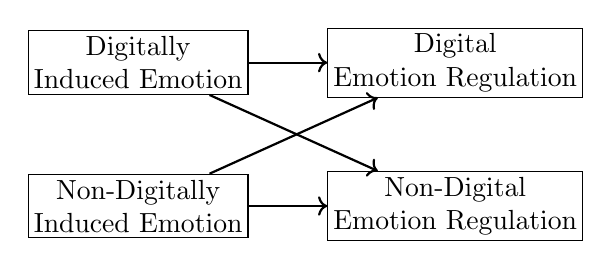
\begin{tikzpicture}[scale=1,transform shape,auto,node distance= 1 cm,
latent/.style={circle,draw,very thick,inner sep=0pt,minimum size=25mm,align=center},
manifest/.style={rectangle,draw,very thick,inner sep=0pt,minimum width=30mm,minimum height=10mm},
paths/.style={->, ultra thick, >=stealth'}]
\node[draw, align=center, minimum width=0.7cm, inner sep=2pt](1) at (0,0){Digitally \\Induced Emotion};
\node[draw, align = center, minimum width=0.7cm, inner sep=2pt](2)[right= of 1]{Digital\\ Emotion Regulation};
\node[draw, align=center, minimum width=0.7cm, inner sep=2pt](3) [below=of 1]{Non-Digitally\\ Induced Emotion};
\node[draw, align=center, minimum width=0.7cm, inner sep=2pt](4)[right=of 3]{Non-Digital \\Emotion Regulation};
\path[->, thick](1)edge(2);
\path[->, thick](3)edge(4);
\path[->, thick](1)edge(4);
\path[->, thick](3)edge(2);
\end{tikzpicture}
  \end{figure}
\end{center}
More research is needed to test and apply this model. In measuring social media usage, researchers distinguish between passive and active social media use. Passive use (scrolling) is associated with worse mental health outcomes than active use (posting) in adolescents \citep{Thorisdottir}. We hypothesized that identification with passive social media use will be linked to poorer emotion regulation skills and increased use of \textit{digital} ER as compared to active social media use. (This is just a preliminary hypothesis for the purposes of this assignment).





\section{Method}
\subsection{Participants}
Participants (\textit{n}= 150) were recruited through local middle and high schools. Participants were majority white (White/Caucasian 35\%, African American 15\%, \textit{these are just placeholders and now that I know how to make the percentage sign show up I will fill this in when I actually have data}). 
\subsection{Materials and Procedure}
{Participants were asked about their time spent on social media, perceptions of their parents' social media use, and their emotion regulation skills.}
\subsubsection{Measure.}Will add a specific measurement here once I select it for my project.

\section{Results}
Table ~\ref{tab:RTmeans} shows descriptive statistics. Significant correlation existed betweeen... (will add in once I actually have the data). The results of a paired-samples t-test indicated that...(will add in once I have the data). 
\\


\begin{table}[h!]
\centering
\caption{\label{tab:RTmeans}Emotion Regulation.}
\begin{tabular}{l l c c c}
 \toprule
                          &              & \multicolumn{3}{c}{Week}\\
  \cmidrule{3-5}
                          &              & {N}           & {Mean}            & {SD}\\
  \cmidrule{3-5}
  \multirow{ 2}{*} & Emotion Regulation &     1008.435    &      986.76     &      859.1     \\
                   & Measure TBD        &     996.23      &      901.67     &      1002.23   \\
  \bottomrule
 \end{tabular}
\end{table}


\newpage
\section{Discussion}
\begin{wrapfigure}{l}{0.5\textwidth}     \centering       
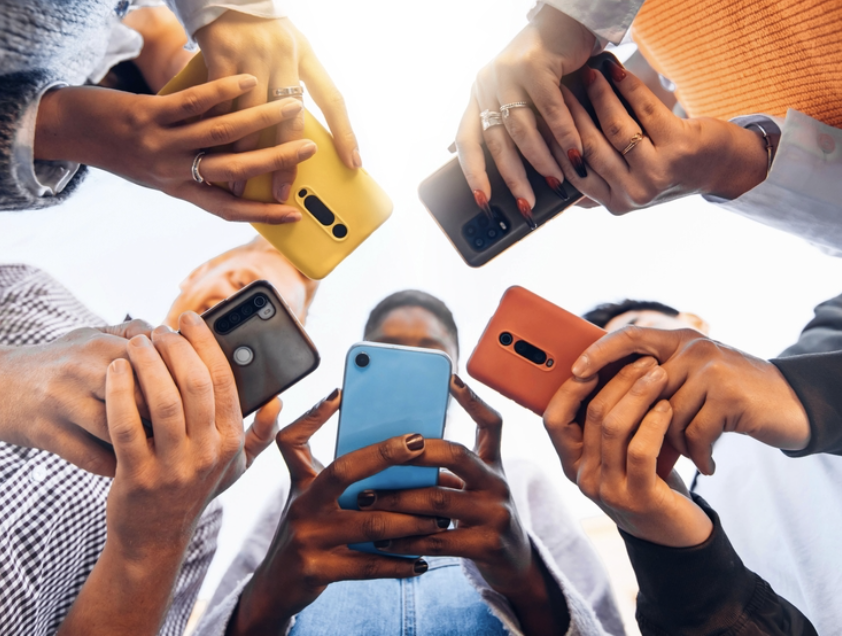
\includegraphics[width=0.4\textwidth]{phones.png}
\caption{\label{fig:latbrain}Teens have increasing access to phones (I will add a more relevant figure here for an actual FYP)}
\end{wrapfigure}

As hypothesized, passive social media use was associated with worse mental health than active social media use. As teens spend more time on social media, and the social connections that are of vital importance to adolescent development move online \citep{hollensteinreview2024}, it is important to understand how adolescents are spending their time in this digital world (see Figure~\ref{fig:latbrain}). The present study contributes to that understanding. Future research should consider using daily diary methods to better capture adolescent emotion and how those emotions are regulated by or simply relate to digital activities. Without understanding these relationships, we cannot understand adolescent development in the modern world.






\bibliography{references.bib}

\end{document}
https://www.overleaf.com/project/64ef8e5b3faa92d4248ddcf9